\section{Method}

\subsection{CTFTiny Benchmark}
% \nanda{TODO}
\label{sec:ctftiny}
\texttt{CTFTiny} is a lightweight evaluation benchmark curated from the full {NYU CTF Bench} to support rapid experimentation while maintaining representative challenge diversity. The motivation behind introducing \texttt{CTFTiny} is the high computational cost associated with running exhaustive evaluations on the full benchmark. Large-scale experiments, such as hyperparameter tuning, model ablations, and sensitivity analysis, are often constrained by prohibitive time and resource requirements of the full set. By reducing the benchmark size while preserving the core characteristics of challenge diversity and complexity, \texttt{CTFTiny} allows more frequent and cost-effective experimentation.

We have selected challenges for \texttt{CTFTiny} using a quantifiable measure of difficulty such that they are neither trivial nor prohibitively difficult. To estimate difficulty, we collate results on NYU CTF Bench from 12 configurations of previous works, namely  \texttt{D-CIPHER}~\cite{udeshi2025d}, and \texttt{CRAKEN}~\cite{shao2025craken}, and use the number of configurations that solved a challenge as empirical measure of difficult. These configurations vary in LLM models, planning strategies, and agentic tools. This empirical measure offers a grounded basis for identifying challenges that require meaningful reasoning and decomposition. Challenge difficulty is classified based on how many of the 12 configurations solved them: 0–3 (hard), 4–6 (moderate), 6–9 (easy), and 9–12 (very easy), where a higher number means the challenge is easier to solve and a lower number means it is harder. Figure~\ref{fig:challengedist} shows the distribution of challenges from \texttt{CTFTiny} based on this empirical measure, demonstrating a healthy spread of challenges across all difficulty levels. 
% This confirms that \texttt{CTFTiny} avoids bias toward trivial or unsolvable tasks, making it well-suited for evaluating both early-stage and mature agentic systems.
The presence of harder challenges ensures the benchmark to stressing model capabilities in reasoning, planning, and strategy adaptation. % This balanced difficulty spectrum strengthens \texttt{CTFTiny} as a reliable, cost-effective proxy for full-scale benchmarking in real-world CTF scenarios. Overall, \texttt{CTFTiny} provides an efficient and focused testbed for benchmarking automated CTF solvers under realistic yet resource-constrained conditions.
\begin{figure}
    \centering
    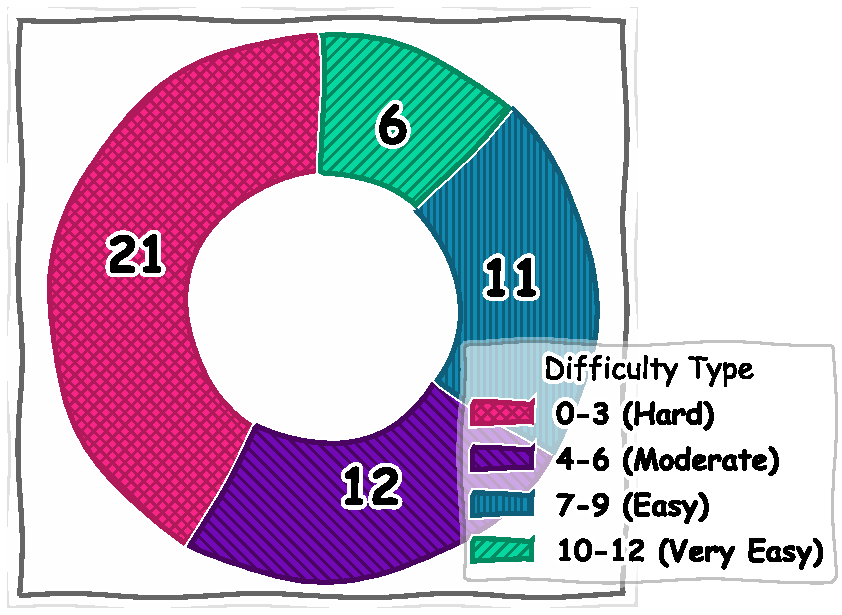
\includegraphics[width=0.75\linewidth]{diagrams/DIST.pdf}
    \caption{Challenge difficulty distribution based on configuration solves, showing a healthy mix of hard, moderate, and easy tasks for robust evaluation.}
    \label{fig:challengedist}
\end{figure}

\subsection{Hyperparameter Tuning}
Our methodological evaluation includes a comprehensive experiment that varies LLM hyperparameters such as temperature, top-$p$, and max tokens to assess their impact on the cybersecurity agent’s performance. These hyperparameters govern the trade‑off between generation diversity and precision; exploring their values ensures our agent maintains robust reasoning, minimizes hallucinations, and optimizes resource usage across diverse challenges. This investigation helps identify robust defaults and guide adaptive parameter tuning for future deployments. By systematically examining these settings, we establish a principled basis for selecting decoding configurations that maximize solution accuracy and stability while controlling computational cost.

\subsection{CTFJudge Agent}

\texttt{CTFJudge} provides a structured evaluation pipeline for LLM‑driven CTF agents, assessing both flag retrieval performance and core cybersecurity competencies. The process begins by transforming expert‑curated writeups into detailed, step‑by‑step summaries that capture each logical decision, underlying intent, key actions, and rationale. In addition the agent’s execution trace, which includes its planning choices, issued commands, observed outcomes, resource usage, and elapsed time, is abstracted into a summary format.

\begin{figure}[b]
\hspace*{-0.15in}
    \centering
    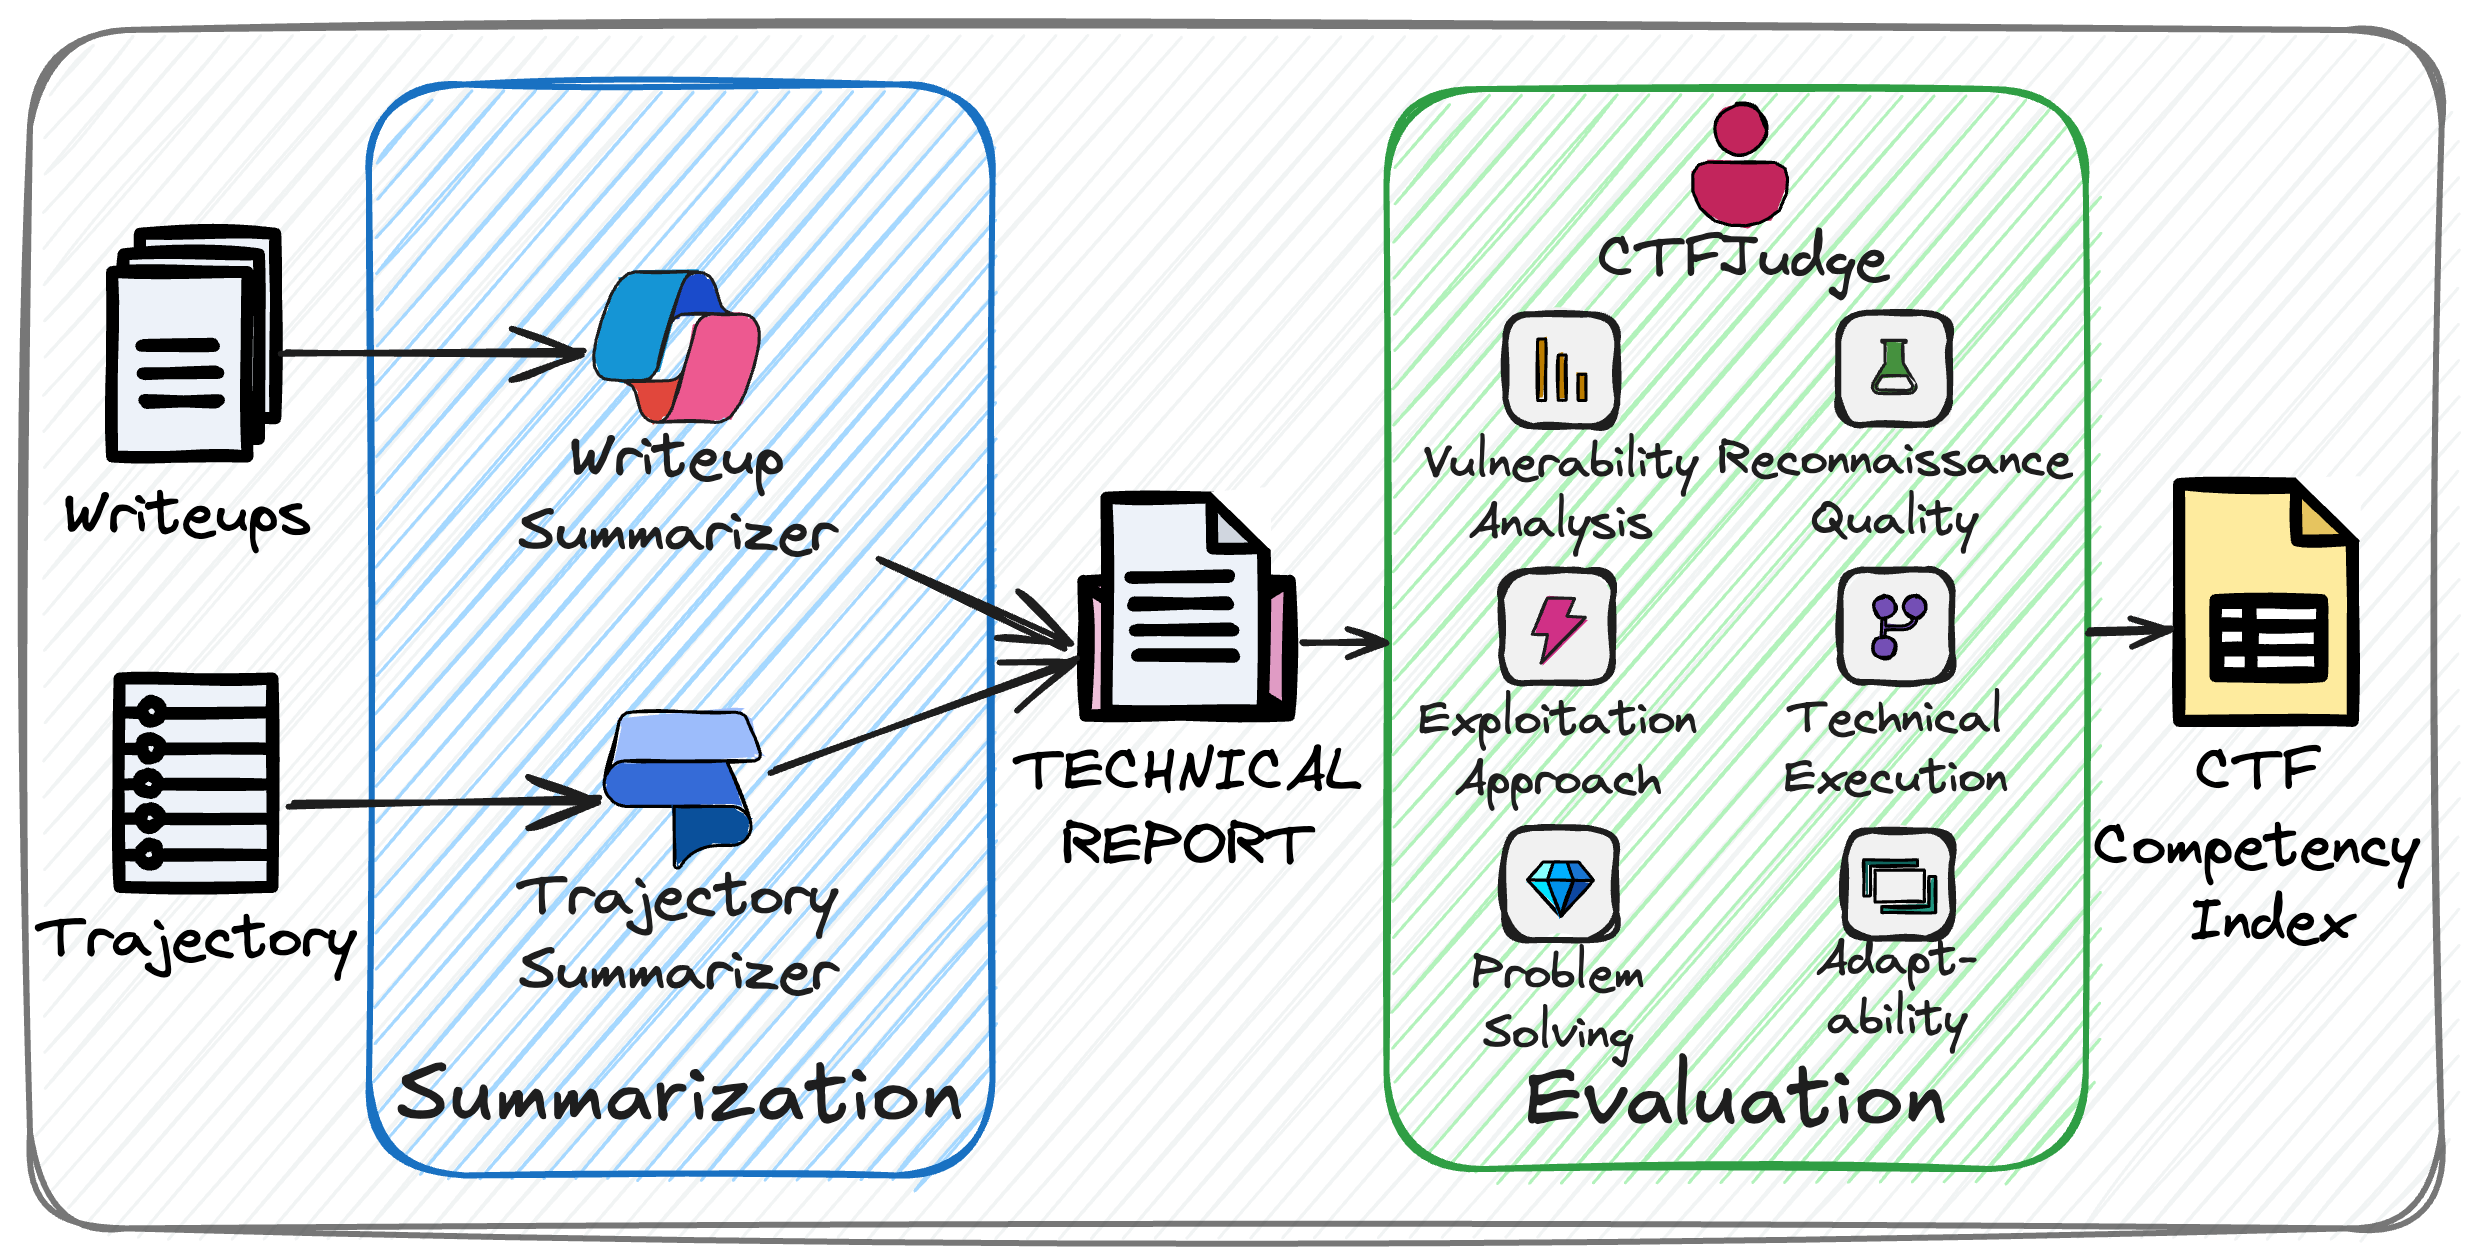
\includegraphics[width=1.1\linewidth]{diagrams/ctf_judge.png}
    \caption{Architecture of the CTFJudge agent, showing how agent trajectories align with expert solutions to generate competency scores and actionable feedback.}
    \label{fig:judge_architecture}
\end{figure}

Once reference and candidate summaries are prepared, \texttt{CTFJudge} produces reference guided 
evaluations along six critical dimensions: vulnerability understanding, reconnaissance thoroughness, exploitation methodology, technical accuracy, efficiency of approach, and adaptability. This granular evaluation produces a quantitative CTF Competency Index (CCI) alongside a narrative report that highlights areas of strength (e.g. comprehensive scanning techniques) and pinpoints opportunities for improvement such as gaps in protocol interpretation or suboptimal command sequencing.

Supporting large-scale, reproducible benchmarking, \texttt{CTFJudge} uses a centralized configuration layer to specify evaluation criteria, model parameters, and factor weights, while built-in error handling and version tracking ensure reliable batch runs. By abstracting implementation details behind clear interfaces, the framework remains extensible, allowing researchers to swap in alternative summarization strategies, integrate real-time telemetry, or add anomaly detection without changing the core evaluation workflow.

% To understand the critical success factors in offensive security agent design, we conduct a comprehensive behavioral analysis by categorizing agent actions into two fundamental patterns: \emph{exploration} and \emph{exploitation}. 

% \emph{Exploration} encompasses reconnaissance activities aimed at understanding the challenge environment, discovering vulnerabilities, and gathering intelligence about target systems—such as directory enumeration, file inspection, and binary analysis. Typical actions include commands like \texttt{ls}, \texttt{cat}, \texttt{strings}, and \texttt{hexdump}. In contrast, \emph{exploitation} represents the execution phase, where agents leverage previously acquired knowledge to perform targeted attacks and achieve objectives.

% This behavioral decomposition addresses a critical limitation in current agentic systems: the tendency toward random, unfocused actions that diminish solving effectiveness. By systematically analyzing decision-making patterns, we investigate whether comprehensive upfront exploration and planning, or reactive exploitation based on immediate observations, serves as the primary driver of CTF challenge success.

% To support this analysis, we implement an automated classification pipeline using multiple approaches. First, we employ rule-based heuristics that categorize commands according to a predefined set of exploration-related actions. Second, we use LLM-based classifiers, including \textsc{GPT-4.1} and \textsc{Claude-3.5-Haiku}, which provide contextual reasoning for each agent action. 

% This multi-classifier framework ensures robust behavioral categorization across diverse challenge types and agent configurations, enabling us to derive actionable insights into optimal coordination strategies and decision-making patterns for effective offensive security automation.

\subsection{CTF Competency Index (CCI)}

To quantify how closely an agent’s trajectory summary \(T\) aligns with a human‑curated gold solution \(G\), \texttt{CTFJudge} employs a weighted combination of \(n\) complementary evaluation factors under its default configuration:
\[
\mathrm{CCI}(T, G)
\;=\;
\sum_{i=1}^{n} w_i\,F_i(T, G),
\quad
\sum_{i=1}^{n} w_i = 1,
\]
where \(n\) denotes the total number of factors and \(F_i\) is the factor that pre-defined. In our initial setup (\(n=6\)), these factors serve as the default evaluation criteria: vulnerability understanding, reconnaissance thoroughness, exploitation methodology, technical accuracy, efficiency of approach, and adaptability. The resulting score lies in \([0,1]\), balancing strategic insight, precision, and operational efficiency for clear comparison and targeted feedback.

These six dimensions align with key stages of offensive cybersecurity. Vulnerability understanding gauges the agent’s ability to identify and interpret system flaws. Reconnaissance thoroughness measures the depth of information gathering. Exploitation methodology evaluates the robustness of attack planning, while technical accuracy ensures commands are executed correctly. Efficiency reflects resource and time optimization, and adaptability captures how the agent handles unexpected scenarios. Together, they provide a balanced benchmark across strategic, technical, and operational fronts, guiding targeted improvements in agent performance.